\section{Short-range correction}
The short-range correction, which takes place immediately after the mesh forces are found using the PM method, is at the heart of the \PThreeM{} algorithm.
Since it scales with a square of the number of particles in each neighborhood, further optimizations are highly desirable.

By Newton's 3rd law, $\mathbf{f}^\text{SR}_{ji} = -\mathbf{f}^\text{SR}_{ij}$, which allows us to do the calculation of the short-range inter-particle force for any pair $(i, j)$ of particles only once, leading to the reduction of the total running time by half.
Informally, the particle $i$ updates its total short-range force $\mathbf{F}^\text{SR}_i$ as well as the total short-range force $\mathbf{F}^\text{SR}_j$ of its neighbor $j$.
To avoid double-counting, the particle $i$ residing in cell $\mathbf{q}$ has to look for its neighbors in a subset $\mathcal{N}$ of the immediate neighborhood of $\mathbf{q}$.
More specifically, define
\begin{equation}\label{eq:n-set}
    \mathcal{N}(\mathbf{q} = (q_1, q_2, q_3)) = \{(q_1+t, q_2-1,q_3+s), (q_1+s, q_2, q_3-1), (q_1-1,q_2,q_3) \;|\; s,t = -1,0,1 \}.
\end{equation}
Thus $|\mathcal{N}| = 13$, which is half of the size of the immediate neighborhood.
The set $\mathcal{N}$ given in \autoref{eq:n-set} is not easy to illustrate.
For the later discussion, it is beneficial to have a clear picture in mind; therefore, we depict its two-dimensional analog in \autoref{fig:n-set-2d}.
\begin{figure}[htp]
    \centering
    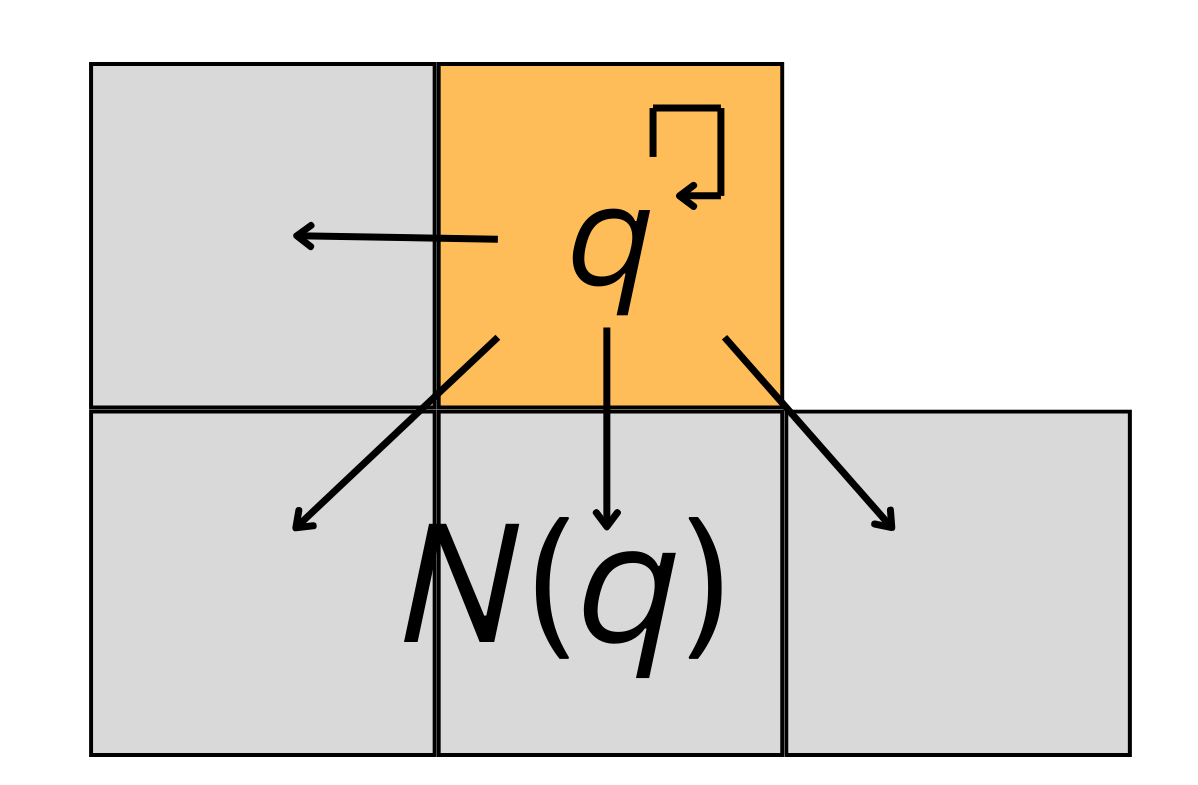
\includegraphics[scale=0.12]{chapters/p3m-method/img/q-neighborhood.png}
    \caption{Set $\mathcal{N}$ in two dimensions.}
    \label{fig:n-set-2d}
\end{figure}

The short-range correction part of the \PThreeM{} method is shown in \autoref{alg:short-range-correction}.
\begin{algorithm}
    \caption{Short-range correction}\label{alg:short-range-correction}
    \begin{algorithmic}[1]
        \ForAll {chaining cell $\mathbf{q}$}
        \ForAll {$\mathbf{q}_n \in \mathcal{N}(\mathbf{q}) \cup \{\mathbf{q}\}$}
        \ForAll {$i \in \text{HOC}(\mathbf{q})$}
        \ForAll {$j \in \text{HOC}(\mathbf{q}_n)$}
        \If {$|y_i - y_j| > r_e$}
        \Break
        \EndIf
        \State \Call{UpdateShortRange}{$i$, $j$, $\mathbf{q}$, $\mathbf{q}_n$}
        \EndFor
        \EndFor
        \EndFor
        \EndFor
    \end{algorithmic}
\end{algorithm}
For each chaining mesh cell $\mathbf{q}$, we compute the pair-wise interactions between the particles in $\mathbf{q}$ and the particles in the chaining mesh cells $\mathbf{q}_n$ from the reduced neighborhood $\mathcal{N}(\mathbf{q})$ \textit{plus} $\mathbf{q}$.
The inclusion of $\mathbf{q}$ allows us to take into account forces between particles within $\mathbf{q}$.

The \textsc{UpdateShortRange} procedure is defined in \autoref{alg:update-short-range-forces}.
\begin{algorithm}
    \caption{Updating short-range forces}\label{alg:update-short-range-forces}
    \begin{algorithmic}[1]
        \Procedure{UpdateShortRange}{$i$, $j$, $\mathbf{q}$, $\mathbf{q}_n$}
        \If {$i = j$}
        \Return
        \EndIf
        \State $\mathbf{r}_{ij} \gets \mathbf{r}_i - \mathbf{r}_j$
        \If {$|\mathbf{r}_{ij}|^2 > r_e^2$}
        \Return
        \EndIf
        \State $r_{ij} \gets |\mathbf{r}_{ij}|$
        \State $\mathbf{\hat{r}}_{ij} \gets \mathbf{r}_{ij} / r_{ij}$
        \State $\mathbf{R}_{ij} \gets -m_i m_j R(r_{ij}) \mathbf{\hat{r}}_{ij}$
        \State $\mathbf{f}^\text{tot} \gets -G m_i m_j / r_{ij}^2 \mathbf{\hat{r}}_{ij}$
        \State $\mathbf{f}^\text{SR}_{ij} \gets \mathbf{f}^\text{tot} - \mathbf{R}_{ij}$
        \State $\mathbf{f}^\text{SR}_{ji} \gets -\mathbf{f}^\text{SR}_{ij}$
        \State $\mathbf{F}^\text{SR}_i \gets \mathbf{F}^\text{SR}_i + \mathbf{f}^\text{SR}_{ij}$
        \If {$\mathbf{q}_n \neq \mathbf{q}$} \Comment{Avoid double-counting in the parent cell}
        \State $\mathbf{F}^\text{SR}_j \gets \mathbf{F}^\text{SR}_j + \mathbf{f}^\text{SR}_{ji}$
        \EndIf
        \EndProcedure
    \end{algorithmic}
\end{algorithm}
In line 2, we exclude self-forces.
The check in line 4 assures that the correction happens only for particles with separation less than the cutoff radius $r_e$.
The pair-wise short-range force is calculated in lines 5--10, with the calculation in line 10 exploiting Newton's third law, as described previously.
The accumulation of total short-range force for a given particle takes place in line 11.
The short-range force is also added to the total short-range force of the other particle in the pair (particle $j$) but only if $\mathbf{q}_n \neq \mathbf{q}$.
This stipulation is crucial, as otherwise, we would be double counting the forces between particles within $\mathbf{q}$.

As suggested in \cite{Hockney1988}, the computational burden of operations in lines 5--8 in \autoref{alg:update-short-range-forces} can be greatly reduced by storing the values of $f^\text{SR}(r) / r = (f^\text{tot}(r) - R(r)) / r$ in a lookup table $T$ at uniform intervals $\Delta^2$ of $[0, r_e^2]$ and interpolating them later.
The schematic depiction of the interpolation is shown in \autoref{fig:sr-force-val-interpolation}.
\begin{figure}[htp]
    \centering
    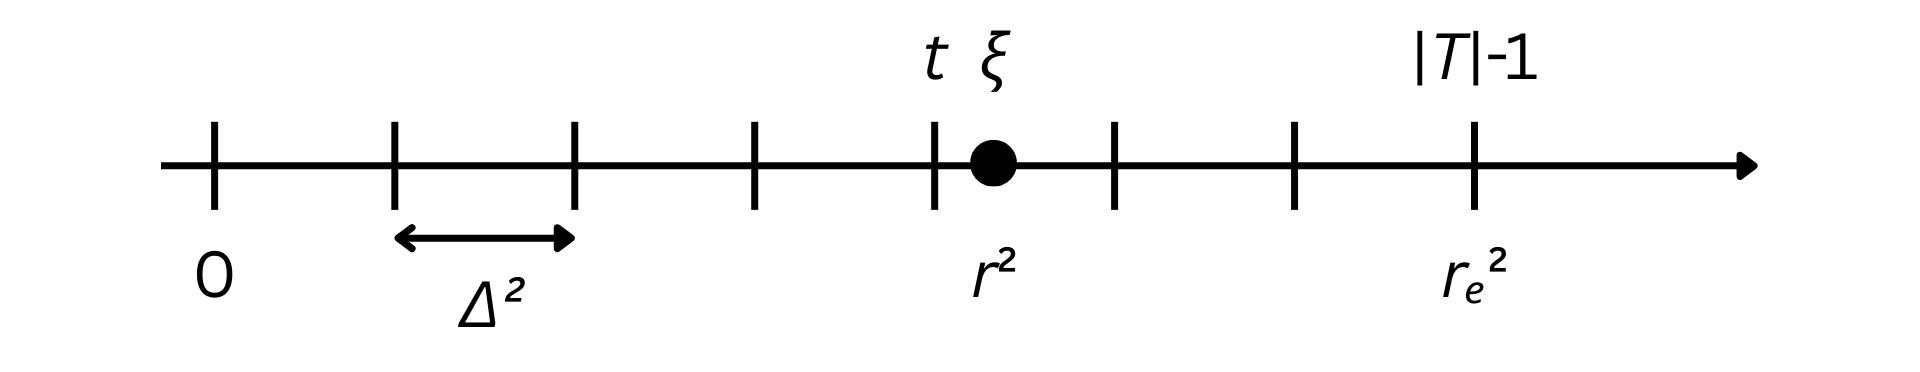
\includegraphics[scale=0.2]{chapters/p3m-method/img/interpolation.png}
    \caption{Interpolation of short-range force values.}
    \label{fig:sr-force-val-interpolation}
\end{figure}
If we define $\xi = r^2 / \Delta^2$ and $t=\lfloor \xi \rfloor$, then
\begin{equation*}
    \frac{f^\text{SR}(r)}{r} \approx T[t]\left(1 - (\xi - t)\right) + T[t+1](\xi - t)
    = T[t] + (\xi - t) (T[t+1] - T[t]).
\end{equation*}
The value $\mathbf{f}^\text{SR}_{ij}$ can then be obtained by multiplying the interpolated quantity $f^\text{SR}(r_{ij})/r_{ij}$ by $G m_i m_j \mathbf{r}_{ij}$, eliminating the use of the square root operations and reducing the total number of floating-point operations to just four.

\subsection{Parallelization}
In our implementation, the procedure outlined in \autoref{alg:short-range-correction} is parallelized by splitting the work done in the outmost loop between some number of threads.
In doing so, extra care has to be taken to avoid data races.
A thread $t$ that is currently processing cell $\mathbf{p}$ and its neighbors (we say that $t$ is \textit{assigned} to $\mathbf{p}$) may ``clash'' with a different thread assigned to a nearby cell $\mathbf{q}$ (because possibly $\mathbf{p} \in \mathcal{N}(\mathbf{q})$).
However, by the construction of the set $\mathcal{N}$, it is possible to split the short-range force into 14 parts, each of which is accessed by only one thread.
For example, consider a particle $i$ in cell $\mathbf{p} = (p_1, p_2, p_3)$ (in other words, $\mathbf{p}$ is the parent cell of $i$).
If thread $t$ is currently assigned to this cell, $t$ will update the part of $\mathbf{F}^\text{SR}_i$ corresponding to updates of $i$ coming from within the same cell as the parent cell of $i$.
Possibly at the same time, thread $t'$ assigned to cell $\mathbf{q} = (p_1+1, p_2, p_3)$ will update a different part of $\mathbf{F}^\text{SR}_i$, i.e., the part corresponding to updates of $i$ coming from the cell ``to the right'' of the parent cell of $i$.
Since only one thread is responsible for updates to particle $i$ coming ``from the right'' (or any other ``direction''), no data races can occur.
This approach presents two major drawbacks.
First, it significantly increases memory usage, requiring storage for an additional $13N$ three-dimensional vectors.
Second, it offers no guarantee of uniform workload distribution across threads.
This imbalance, combined with the substantial variation in operations performed by individual threads, leads to severe thread divergence, rendering the parallelization scheme unsuitable for GPU execution and making it only applicable to the CPU implementation.
Despite these shortcomings, tests performed on our machine (utilizing the maximum number of concurrent threads supported, equal to 12) yielded more than four-fold speedup compared to the single-threaded implementation in a typical simulation.
The results of a performance test for a typical simulation are shown in \autoref{fig:p3m-time-threads}.
\begin{figure}[htp]
    \centering
    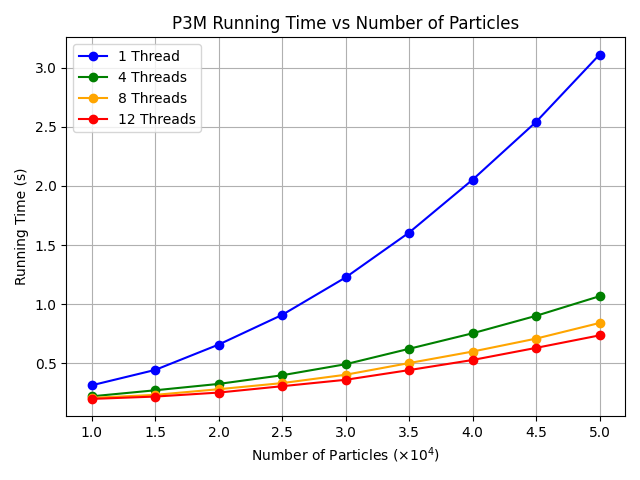
\includegraphics[scale=0.5]{chapters/p3m-method/img/p3m_threads.png}
    \caption{Running time per iteration of the \PThreeM{} method using different numbers of threads.}
    \label{fig:p3m-time-threads}
\end{figure}
As illustrated in the figure, increasing the number of threads initially improves performance, but beyond a certain point, the gains level off.
This is because the system reaches the limit of its physical cores (six in our case) after which additional threads do not contribute meaningfully.
Further increasing the thread count introduces overhead from context switching, which ultimately becomes the dominant performance bottleneck.
